\documentclass[12pt]{article}

\usepackage{geometry, subfiles}
\usepackage{amsmath, amssymb}
\usepackage{booktabs, longtable, siunitx}
\usepackage{graphicx,subcaption}
%\graphicspath{/Users/wonjun/Dropbox/Emory/ECON771_health2/assignments/assignment3/output/}

\title{Assignment 3}
\author{Wonjun Choi}

\begin{document}
\maketitle
\begin{itemize}
	\item[1.] The descriptive statistics are given in Table \ref{tab:descstat}
	
	\subfile{../output/tab_descstat.tex}

	
	\item[2.] Figure \ref{fig:rdplot} shows a RD plot of  monthly premium and logged enrollment state in 2006.
	\begin{figure} [ht]
		\centering
		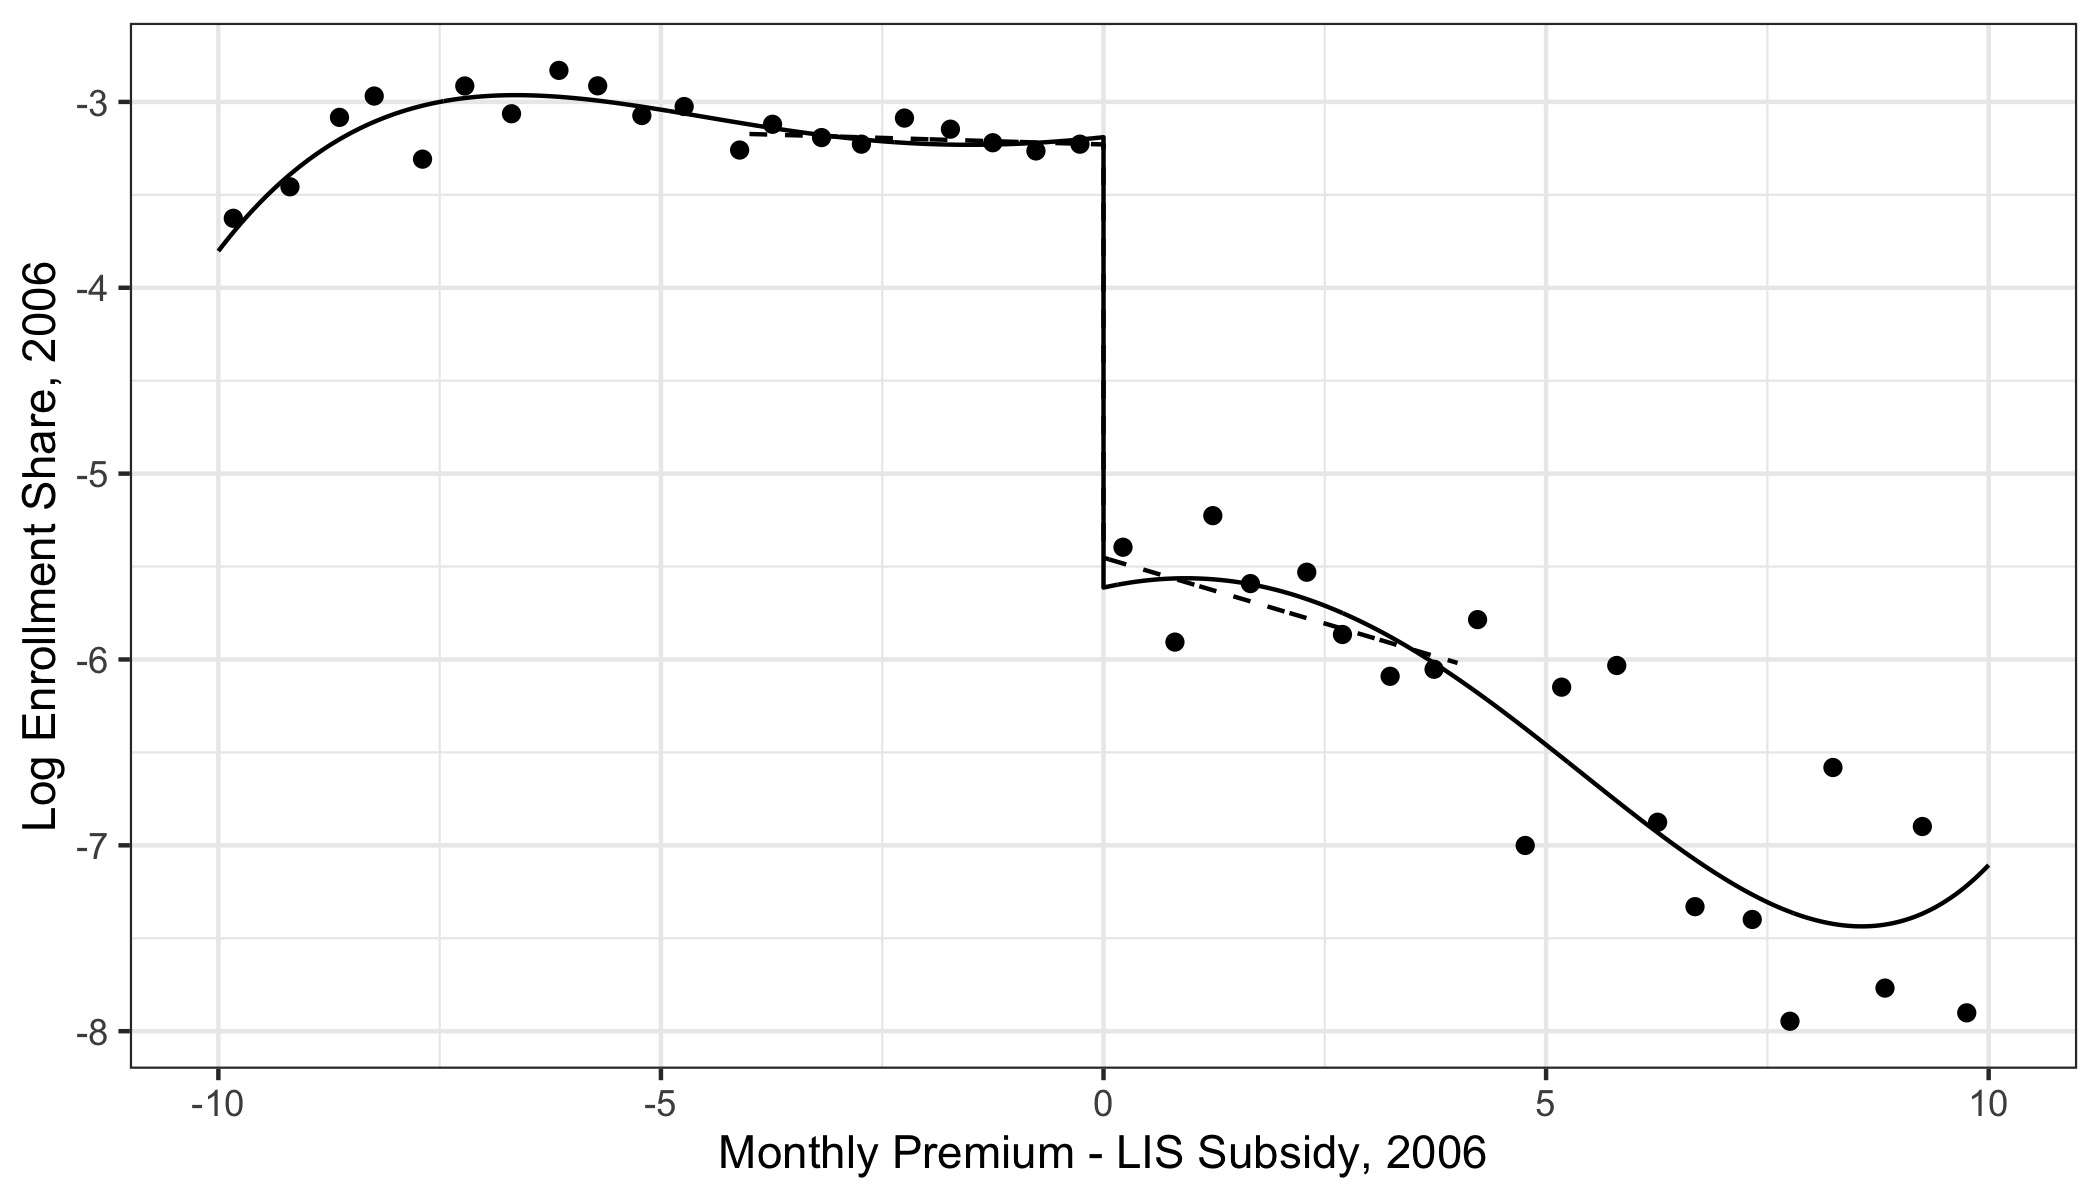
\includegraphics[scale=0.15]{../output/fig_rdplot.jpg}
		\caption{The Effect of 2006 Benchmark Status on 2006 Enrollment}
		\label{fig:rdplot}
	\end{figure}

\item[3.] The RD plot using different number of partitions are given in Figure \ref{fig:bins}. I am not sure if the figures convey different information. They all seem to show sharp discontinuity around the benchmark.
    \begin{figure} [ht]
    	\begin{subfigure}{.5\textwidth}
    		\centering
    		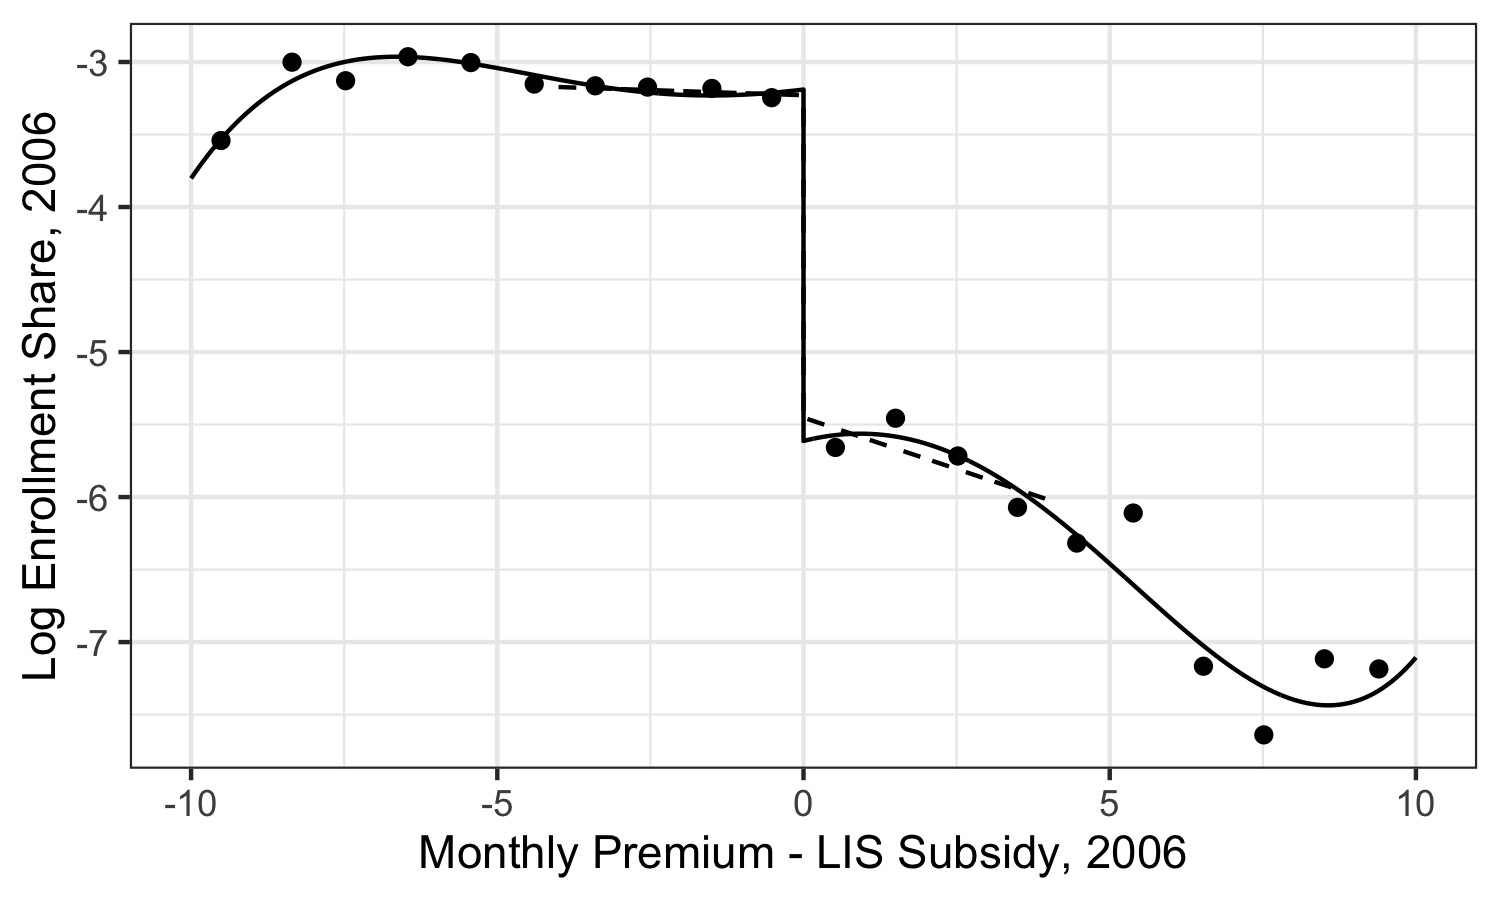
\includegraphics[scale=0.14]{../output/fig_rdplot_j10.jpg}
    		\caption{J=10}
    	\end{subfigure}%
       \begin{subfigure}{.5\textwidth}
    	\centering
    	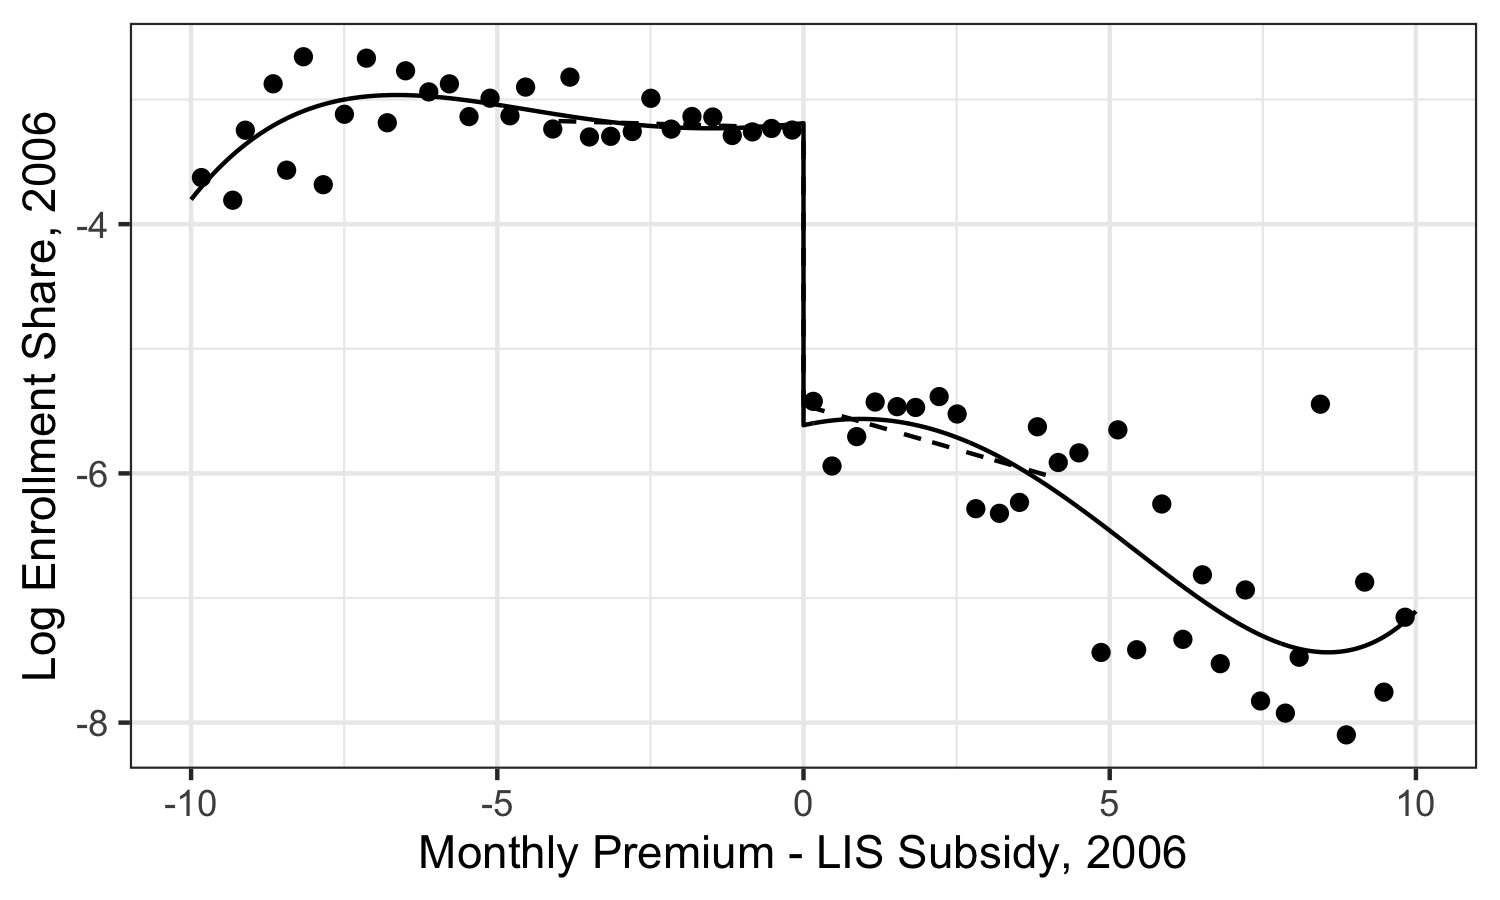
\includegraphics[scale=0.14]{../output/fig_rdplot_j30.jpg}
    	\caption{J=30}
       \end{subfigure}
        \caption{Different bin size}
        \label{fig:bins}
    \end{figure}

\item[4.] The RD plot with the optimal number of partition is presented in Figure \ref{fig:binopt}. The optimal numbers of bins were $J_-=15$ and $J_+=17$.
\begin{figure} [ht]
	\centering
	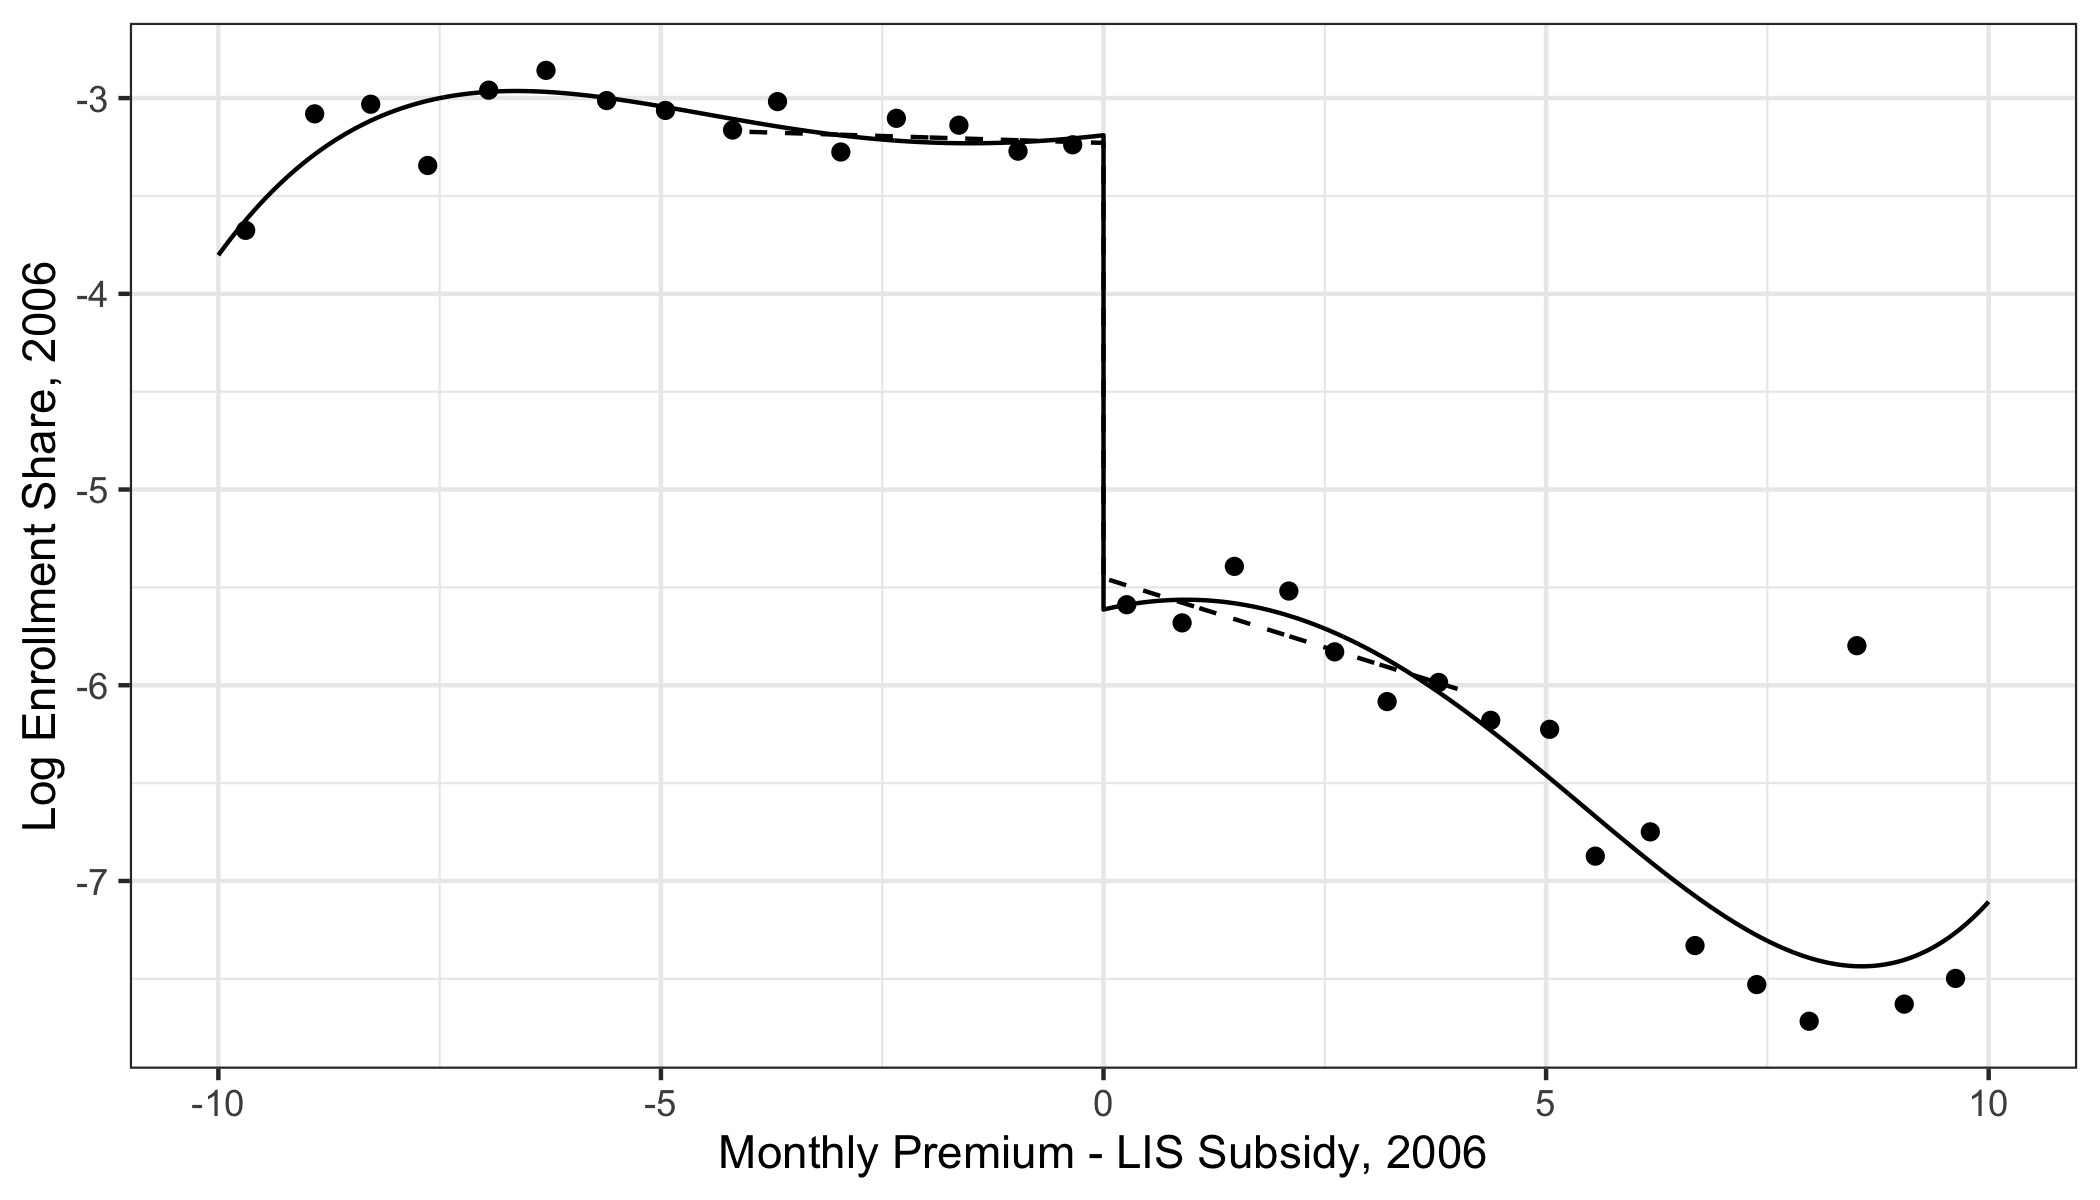
\includegraphics[scale=0.15]{../output/fig_binopt.jpg}
	\caption{RD plot with the optimal number of partition ($J_-=15$, $J_+=17$)}
	\label{fig:binopt}
\end{figure}

\item[5.] The figure of the density of the running variable is displayed in Figure \ref{fig:density}.
\begin{figure}
	\centering
	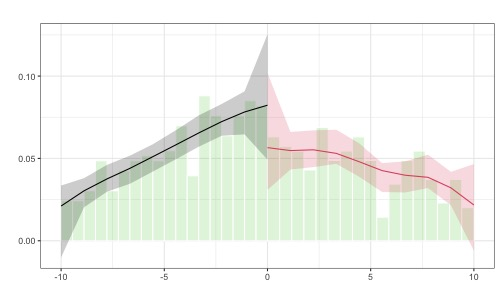
\includegraphics[scale=0.8]{../output/fig_density.jpg}
	\caption{Probability density of the running variable}
	\label{fig:density}
\end{figure}
The density of the left limit was higher than the density of the right limit, but the difference was not statistically significant.

\item[6.] The regression results are presented in Table \ref{tab:panel1} and \ref{tab:panel2}. Table 3 shows the result of local quadratic regression.
\subfile{../output/tab_panel1}
\subfile{../output/tab_panel2}

\item[7.] The regression result using the CE-optimal bandwidth (Calonico et al., 2020) is given in Table \ref{tab:rdrobust_panel1} and Table \ref{tab:rdrobust_panel2}
\subfile{../output/tab_rdrobust_panel1}
\subfile{../output/tab_rdrobust_panel2}
The bandwidth in question 6 was uniformly 4. However, the CE-optimal bandwidth was by far smaller than 4. Overall coefficients didn't change much in year 2006, 2007, and 2008, but the coefficients were significantly different in year 2009, 2010.

\item[8.] Table \ref{tab:iv} shows the 2SLS result. The result implies that the premium does not become higher as the plan becomes market dominant.

\begin{table}[ht]
	\subfile{../output/tab_iv}
	\caption{The Effect of Enrollment Share on Premium}
	\label{tab:iv}
\end{table}


\item[9.] The results were robust to the choice of bandwidth. Table 4 in Ericson (2014) shows the plan that survived longer has higher premium, suggesting that insurers might exploit profit from consumer inertia. However, the IV results of question 8 shows market share in fact has no effect on premium, where it should have had a positive correlation if the invest-then-harvest were true. 

\item[10.] While RD was intuitively straightforward, the theory and coding behind was quite invovled to me. However, I don't actually see there is much gain in using more sophisticated technique. I am not sure how much they can improve empirical findings.


\end{itemize}

\end{document}